\chapter{Discrimination}

\begin{description}
    \item[Disparate treatment] \marginnote{Disparate treatment}
        The outcome of an algorithm is based on protected features.

    \item[Disparate impact] \marginnote{Disparate impact}
        The outcome of an algorithm that uses neutral features is disproportionate against certain groups without an acceptable reason.
\end{description}


\section{Biased data}


\subsection{Historical bias}

\begin{description}
    \item[Historical bias] \marginnote{Historical bias}
        System trained on intrinsically biased data will reproduce the same biased behavior.

        \begin{remark}
            Data can be biased because it comes from past human judgement or by the hierarchies of society (e.g., systems working on marginalized languages will most likely have lower performance compared to a widespread language).
        \end{remark}
\end{description}

\begin{example}[Amazon AI recruiting tool]
    Tool that Amazon was using in the past to review job applications. It was heavily biased towards male applicants and, even with the gender removed, it was able to infer it from the other features.

    \begin{figure}[H]
        \centering
        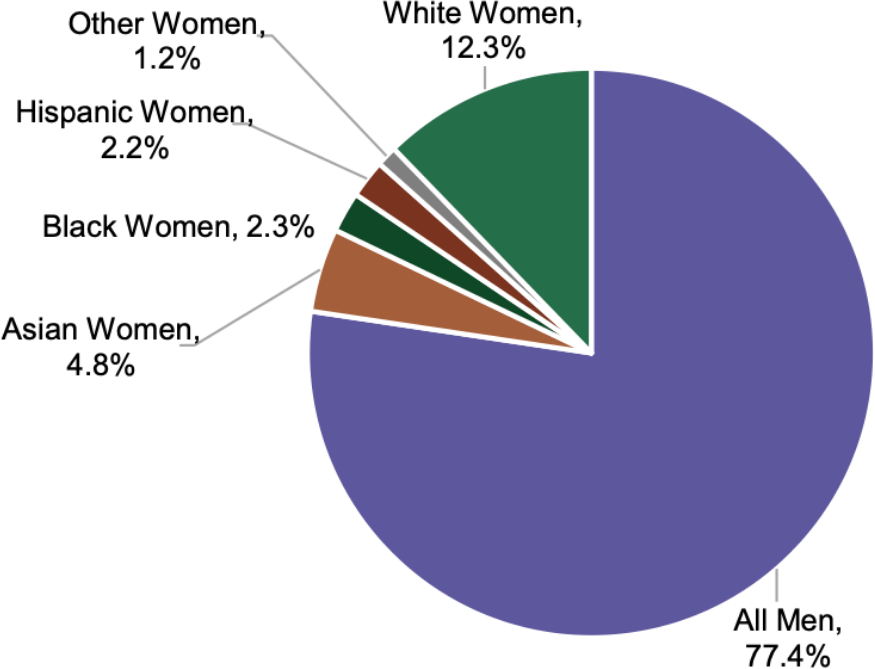
\includegraphics[width=0.3\linewidth]{./img/tech_workforce.png}
        \caption{Tech companies workforce in the US}
    \end{figure}
\end{example}

\begin{example}[UK AI visa and asylum system]
    System used by the UK government to assess visa and asylum applications. It was found that:
    \begin{itemize}
        \item The system ranked applications based on nationality.
        \item Applicants from certain countries were automatically flagged as high risk.
    \end{itemize}
\end{example}

\begin{example}[Generative AI]
    Prompting Stable Diffusion to generate the image of a \texttt{ceo} and a \texttt{nurse} highlights the gender and ethnicity bias of the training data.

    \begin{figure}[H]
        \centering
        \begin{subfigure}{0.5\linewidth}
            \centering
            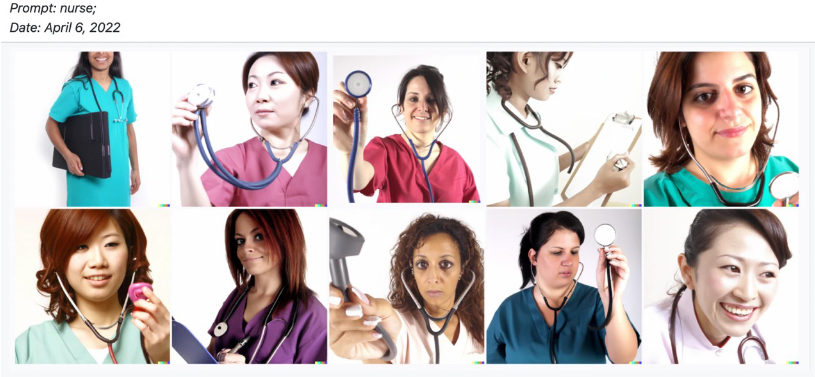
\includegraphics[width=\linewidth]{./img/stable_diffusion_nurse.png}
        \end{subfigure}
        \hfill
        \begin{subfigure}{0.4\linewidth}
            \centering
            
\includegraphics[width=\linewidth]{./img/stable_diffusion_ceo.png}
        \end{subfigure}
    \end{figure}

    Also, other systems (e.g., Gemini) included constraints to favor diversity resulting in unexpected results.

    \begin{figure}[H]
        \centering
        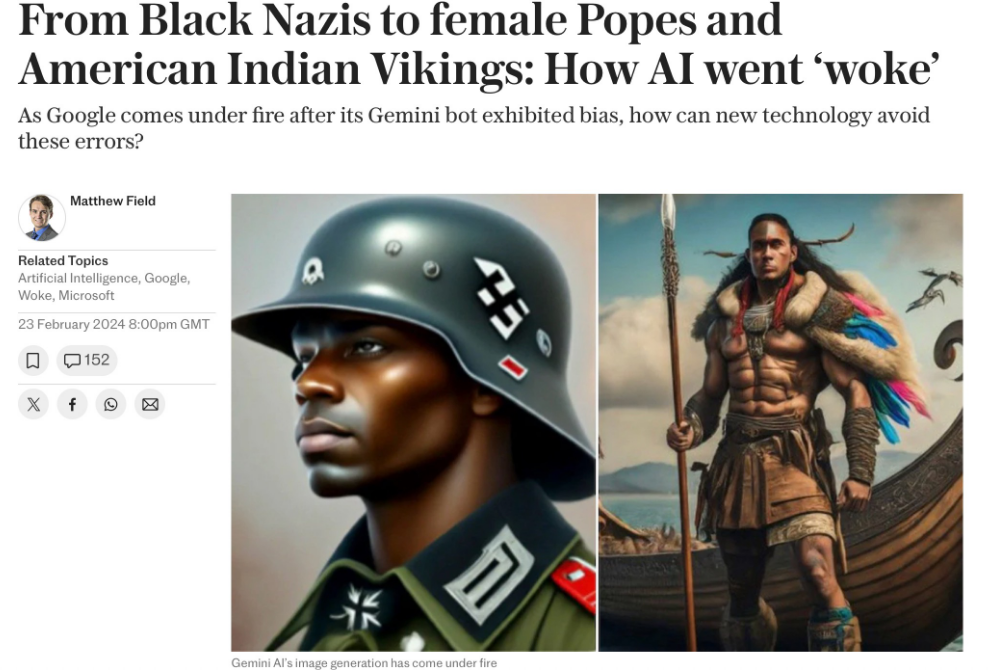
\includegraphics[width=0.45\linewidth]{./img/gemini_diversity.png}
    \end{figure}

    In the context of language models, some systems implement a refusal mechanism to prevent a biased response. However:
    \begin{itemize}
        \item Using a different prompt of the same topic might bypass the filter.
        \item Refusal might be applied unequally depending on demographics or domain.
    \end{itemize}
\end{example}


\subsection{Proxy variables}

\begin{description}
    \item[Proxy variable] \marginnote{Proxy variable}
        Neutral feature that is connected to a protected one resulting in a disparate impact on a certain group.
\end{description}

\begin{example}[Disaster relief allocation system]
    A system that predicts which communities need assistance based on past insurance claims is biased as it is a proxy for socioeconomic conditions: low-income communities often have lower insurance coverage and therefore will be disadvantaged by this system.
\end{example}

\begin{example}[Optum healthcare algorithm]
    System used in US hospitals to predict which patients would benefit from additional resources. It was trained on historical data and it was found out that it was using the past healthcare cost data as a proxy to assess medical needs.

    Due to historical disparity in accessing healthcare, this would cause a disparate impact on minorities that were unable to afford healthcare.
\end{example}

\begin{example}[Hurricane Katrina and racial disparities]
    Due to historical racial segregation, the neighborhoods of many US cities can be divided by ethnicity. When Hurricane Katrina hit New Orleans, it mainly damaged the side of the city mostly lived by low-income communities. However, the evacuation plans assumed the availability of private vehicles and shelters were mostly built in the wealthier areas. Also, federal aid arrived quicker for wealthier communities and many low-income residences were never rebuilt.

    An AI system trained on these data would reproduce the same behavior using the area one lives as a proxy.
\end{example}


\subsection{Biases embedded in predictors}

\begin{description}
    \item[Bias embedded in predictors] \marginnote{Bias embedded in predictors}
        A system that uses favorable features that only a certain group has.
\end{description}

\begin{example}[House allocation in Los Angeles]
    VI-SPDAT is a system used in Los Angeles to distribute housing resources to homeless. As it relied on self-reported information, it was favoring those with higher literacy levels.
\end{example}


\subsection{Unbalanced samples}

\begin{description}
    \item[Unbalanced samples] \marginnote{Unbalanced samples}
        The dataset does not reflect the statistical composition of the population.
\end{description}

\begin{example}
    Due to the lack of data of certain groups, a system to predict diseases will be more inaccurate towards minorities.
\end{example}



\section{Algorithm choice}


\subsection{Aggregation bias problem}

\begin{description}
    \item[Aggregation bias problem] \marginnote{Aggregation bias problem}
        System that has good results overall but with poor performance for specific groups.
\end{description}

\begin{example}
    A system to predict the distribution of humanitarian aid trained on past successful data can present aggregation bias due to geographical data as a large part of the training data will most likely come from well established urban areas.
\end{example}


\subsection{Different base rates}

\begin{description}
    \item[Base rate/prior probability] \marginnote{Base rate/prior probability}
        Proportion of samples belonging to a certain class.
\end{description}

\begin{example}[COMPAS system]
    COMPAS is a system used by US courts to determine the risk of recidivism (high, medium, low).

    \begin{description}
        \item[Loomis case]
            E. Loomis was a defendant that according to COMPAS had a high risk of recidivism and was sentenced to 6 years in prison. The decision was appealed by Loomis as COMPAS has the following issues:
            \begin{itemize}
                \item Its functioning is unknown,
                \item Its validity cannot be verified,
                \item It discriminates on gender and ethnicity,
                \item Statistical predictions violate the right to individualized decisions.
            \end{itemize}

            The Supreme Court of Wisconsin rejected the argument and stated that:
            \begin{itemize}
                \item Statistical algorithms do not violate the right to individualized decisions as they are used to enhance a judge's evaluation,
                \item Gender is necessary to achieve statistical accuracy,
                \item Judges should be informed about the possibility of racial discrimination by COMPAS.
            \end{itemize}

        \item[ProPublica and Northpointe studies]
            ProPublica, a non-profit organization, published a study on the accuracy and fairness of COMPAS by comparing the predicted recidivism rates of $\num{11757}$ defendants and the actual rates between 2013 and 2014. Results found out that:
            \begin{itemize}
                \item The overall accuracy is moderate-low ($61.2\%$),
                \item Black defendants were more likely labeled with a high level of risk, leading to a higher probability of high risk misclassification ($45\%$ blacks vs $23\%$ whites).
                \item White defendants were more likely labeled with a low level of risk, leading to a higher probability of low risk misclassification ($48\%$ whites vs $28\%$ blacks).
            \end{itemize}

            Northpointe, the software house of COMPAS, stated that ProPublica made several statistical and technical errors as:
            \begin{itemize}
                \item The accuracy of COMPAS is higher that human judgement.
                \item The general recidivism risk scale is equally accurate for blacks and whites,
                \item COMPAS is compliant with the principle of fairness and does not implement racial discrimination.
            \end{itemize}
    \end{description}

    \indenttbox
    \begin{remark}[Decision workflow]
        A decision system can be represented in three steps:
        \begin{enumerate}
            \item Assign a predictive score (i.e., compute likelihood). In this step, unfairness can be caused by using protected features, biased data, a proxy, \dots
            \item Classify the score based on some thresholds. In this step, unfairness can be caused by the choice of the threshold.
            \item Make the decision. In this step, unfairness can be caused by how the value is used.
        \end{enumerate}
        \begin{figure}[H]
            \centering
            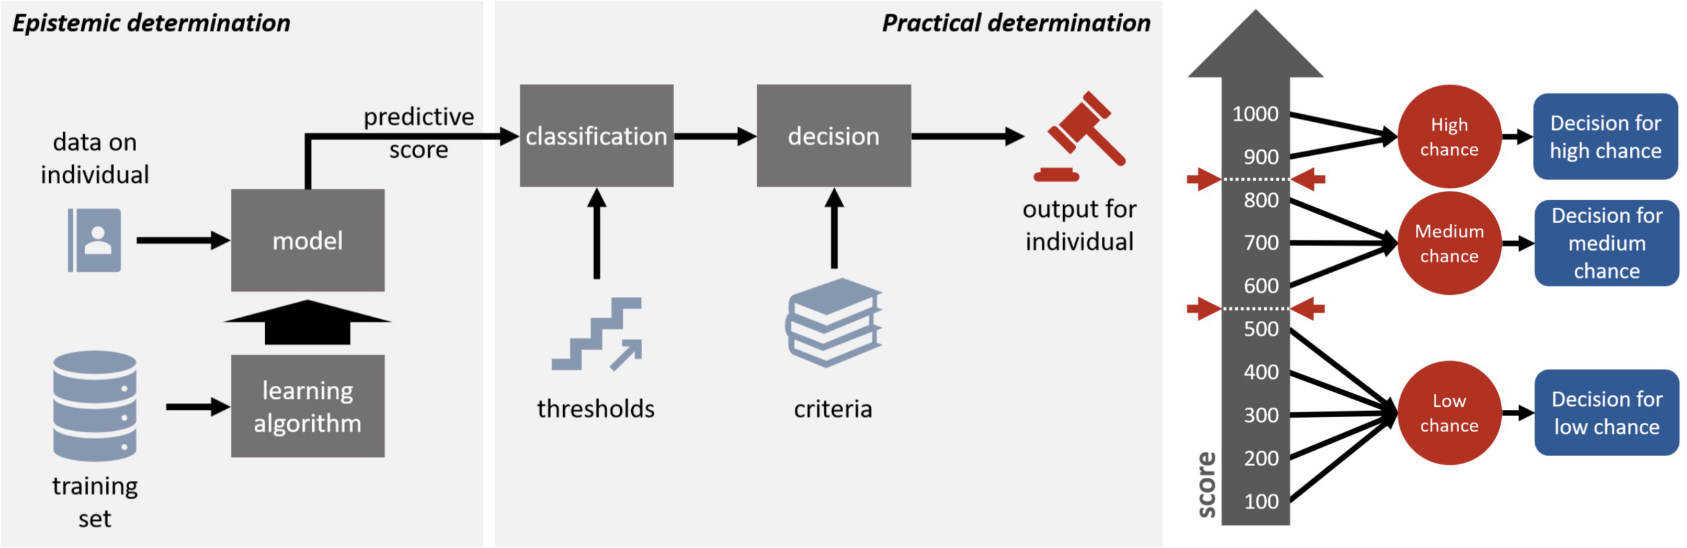
\includegraphics[width=0.8\linewidth]{./img/decision_anatomy.png}
        \end{figure}
    \end{remark}

    \begin{description}
        \item[SAPMOC case]
            SAPMOC is a toy example that predicts recidivism only based on whether the defendant has a previous criminal record. Assume that:
            \begin{itemize}
                \item $80\%$ of previous offenders recidivate and the remaining do not.
                \item $20\%$ of first time offenders recidivate and the remaining do not.
                \item The training data is composed of 3000 defendants divided into 1500 blues (1000 previous offenders) and 1500 greens (500 previous offenders).
            \end{itemize}

            Therefore, the ground-truth aggregated outcomes are:
            \begin{center}
                \footnotesize
                \begin{tabular}{c|cc}
                    \toprule
                                            & \textbf{Has record} & \textbf{No record} \\
                    \midrule
                    \textbf{Recidivism}     & 1200 ($80\%$) & 300 ($20\%$) \\
                    \textbf{No recidivism}  & 300 ($20\%$) & 1200 ($80\%$) \\
                    \bottomrule
                \end{tabular}
            \end{center}
            
            Assume that SAPMOC's predictions are:\\[-1.5em]
            \begin{minipage}{0.48\linewidth}
                \begin{table}[H]
                    \caption{Aggregated predictions}
                    \footnotesize
                    \begin{tabular}{c|cc}
                        \toprule
                                                & \textbf{Has record} & \textbf{No record} \\
                        \midrule
                        \textbf{Recidivism}     & 1500 & 0 \\
                        \textbf{No recidivism}  & 0 & 1500 \\
                        \bottomrule
                    \end{tabular}
                \end{table}
            \end{minipage}
            \hfill
            \begin{minipage}{0.48\linewidth}
                \begin{table}[H]
                    \caption{Group-wise confusion matrix}
                    \footnotesize
                    \begin{tabular}{c|ccc|ccc}
                        \toprule
                        & \textbf{Pos.} & \texttt{TP} & \texttt{FP} & \textbf{Neg.} & \texttt{TN} & \texttt{FN} \\ 
                        \midrule
                        \textbf{Blues} & 1000 & 800 & 200 & 500 & 400 & 100 \\ 
                        \textbf{Greens} & 500 & 400 & 100 & 1000 & 800 & 200 \\
                        \bottomrule
                    \end{tabular}
                \end{table}
            \end{minipage}

            The base rates are then computed as:
            \begin{center}
                \footnotesize
                \begin{tabular}{c|cc}
                    \toprule
                        & $\textbf{Base rate}_\textbf{pos}$ $\frac{\texttt{TP}+\texttt{FN}}{\texttt{TP}+\texttt{FN}+\texttt{FP}+\texttt{TN}}$ 
                        & $\textbf{Base rate}_\textbf{neg}$ $\frac{\texttt{TN}+\texttt{FP}}{\texttt{TP}+\texttt{FN}+\texttt{FP}+\texttt{TN}}$ \\
                    \midrule
                        \textbf{Blues} & $\frac{900}{1500} = 60\%$ & $\frac{600}{1500} = 40\%$ \\
                        \textbf{Greens} & $\frac{600}{1500} = 40\%$ & $\frac{900}{1500} = 60\%$ \\
                    \bottomrule
                \end{tabular}
            \end{center}

            Note that the overall accuracy is the same for each group:
            \begin{center}
                \footnotesize
                \begin{tabular}{c|c}
                    \toprule
                        & \textbf{Accuracy} $\frac{\texttt{TP}+\texttt{TN}}{\texttt{TP}+\texttt{FN}+\texttt{FP}+\texttt{TN}}$ \\
                    \midrule
                        \textbf{Blues} & $80\%$ \\
                        \textbf{Greens} & $80\%$ \\
                    \bottomrule
                \end{tabular}
            \end{center}
    \end{description}
\end{example}

\begin{description}
    \item[Fairness criteria]
        The main fairness criteria are the following:
        \begin{description}
            \item[Statistical parity] \marginnote{Statistical parity}
                Each group should have an equal proportion of positive and negative predictions.
                \begin{example}[SAPMOC]
                    SAPMOC does not satisfy statistical parity:
                    \begin{center}
                        \footnotesize
                        \begin{tabular}{c|cc}
                            \toprule
                                & \textbf{Predicted pos.} $\frac{\texttt{TP}+\texttt{FP}}{\texttt{TP}+\texttt{FN}+\texttt{FP}+\texttt{TN}}$ 
                                & \textbf{Predicted neg.} $\frac{\texttt{TN}+\texttt{TN}}{\texttt{FN}+\texttt{FN}+\texttt{FP}+\texttt{TN}}$ \\
                            \midrule
                                \textbf{Blues} & $67\%$ & $33\%$ \\
                                \textbf{Greens} & $33\%$ & $67\%$ \\
                            \bottomrule
                        \end{tabular}
                    \end{center}
                \end{example}

            \item[Equality of opportunity/true positive rate] \marginnote{Equality of opportunity/true positive rate}
                The members sharing the same features between different groups should be treated equally (i.e., same recall).
                \begin{example}[SAPMOC]
                    SAPMOC does not satisfy equality of opportunity:
                    \begin{center}
                        \footnotesize
                        \begin{tabular}{c|cc}
                            \toprule
                                & \textbf{Recall pos.} $\frac{\texttt{TP}}{\texttt{TP}+\texttt{FN}}$ 
                                & \textbf{Recall neg.} $\frac{\texttt{TN}}{\texttt{TN}+\texttt{FP}}$ \\
                            \midrule
                                \textbf{Blues} & $89\%$ & $67\%$ \\
                                \textbf{Greens} & $67\%$ & $89\%$ \\
                            \bottomrule
                        \end{tabular}
                    \end{center}
                \end{example}

            \item[Calibration] \marginnote{Calibration}
                The proportion of correct predictions should be equal for each class within each group (i.e., same precision).
                \begin{example}[SAPMOC]
                    SAPMOC satisfies calibration:
                    \begin{center}
                        \footnotesize
                        \begin{tabular}{c|cc}
                            \toprule
                                & \textbf{Precision pos.} $\frac{\texttt{TP}}{\texttt{TP}+\texttt{FP}}$ 
                                & \textbf{Precision neg.} $\frac{\texttt{TN}}{\texttt{TN}+\texttt{FN}}$ \\
                            \midrule
                                \textbf{Blues} & $80\%$ & $80\%$ \\
                                \textbf{Greens} & $80\%$ & $80\%$ \\
                            \bottomrule
                        \end{tabular}
                    \end{center}
                \end{example}

            \item[Conditional use error/false rate] \marginnote{Conditional use error/false rate}
                The proportion of incorrect predictions should be equal for each class within each group.
                \begin{example}[SAPMOC]
                    SAPMOC satisfies conditional use error:
                    \begin{center}
                        \footnotesize
                        \begin{tabular}{c|cc}
                            \toprule
                                & \textbf{False rate pos.} $\frac{\texttt{FP}}{\texttt{TP}+\texttt{FP}}$ 
                                & \textbf{False rate neg.} $\frac{\texttt{FN}}{\texttt{TN}+\texttt{FN}}$ \\
                            \midrule
                                \textbf{Blues} & $20\%$ & $20\%$ \\
                                \textbf{Greens} & $20\%$ & $20\%$ \\
                            \bottomrule
                        \end{tabular}
                    \end{center}
                \end{example}

            \item[Treatment equality] \marginnote{Treatment equality}
                The error ratio of positive and negative predictions should be equal across all groups.
                \begin{example}[SAPMOC]
                    SAPMOC does not satisfy treatment equality:
                    \begin{center}
                        \footnotesize
                        \begin{tabular}{c|cc}
                            \toprule
                                & \textbf{Error pos.} $\frac{\texttt{FP}}{\texttt{FN}}$ 
                                & \textbf{Error neg.} $\frac{\texttt{FN}}{\texttt{FP}}$ \\
                            \midrule
                                \textbf{Blues} & $200\%$ & $50\%$ \\
                                \textbf{Greens} & $50\%$ & $200\%$ \\
                            \bottomrule
                        \end{tabular}
                    \end{center}
                \end{example}
        \end{description}

        \begin{remark}
            There are many other fairness criteria that are correlated to those above.
        \end{remark}

        \begin{remark}
            There is a conflict between individual and group fairness so that not all criteria can be satisfied at once.
        \end{remark}
\end{description}

\begin{description}
    \item[Handling different base rates] \phantom{}
        \begin{description}
            \item[Do nothing] \marginnote{Do nothing}
                Accept that different groups are actually associated to different probabilities.

            \item[Modify the threshold for everyone] \marginnote{Modify the threshold for everyone}
                Raise (or decrease) the threshold to diminish the favorable classification for everyone (affecting more the groups with a higher base rate).

            \item[Change the decision for everyone] \marginnote{Change the decision for everyone}
                Adopt alternative measures based on the classification results or use different thresholds depending on the group.

                \begin{remark}
                    Using different thresholds might still lead to discrimination. It makes sense in cases that require an affirmative action to increase diversity.
                \end{remark}
        \end{description}
\end{description}

\begin{example}[SAPMOC II]
    SAPMOC extended to multiple features and an output in $[0, 1]$. It is possible to represent the relationship between the output score and the likelihood of recidivism as densities:
    \begin{descriptionlist}
        \item[Recidivism density]
            Function of the score such that the area under the curve between $[s', s'']$ is the number of recidivists associated to a score in that interval.

        \item[Non-recidivism density]
            Function of the score such that the area under the curve between $[s', s'']$ is the number of non-recidivists associated to a score in that interval.
    \end{descriptionlist}

    \begin{figure}[H]
        \centering
        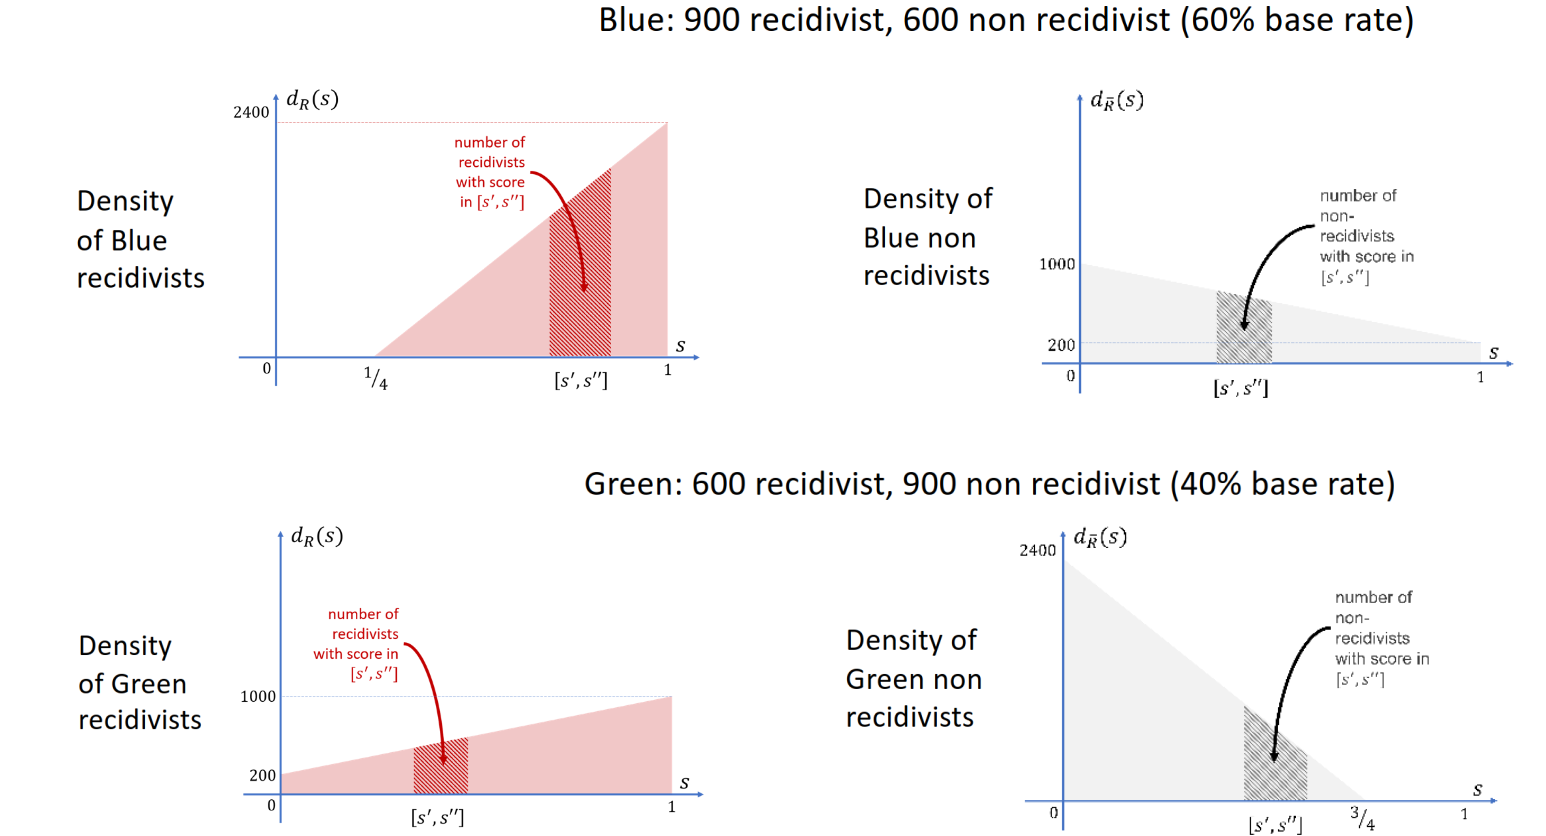
\includegraphics[width=0.75\linewidth]{./img/sapmoc_density.png}
    \end{figure}

    If the same threshold is applied for both groups, SAPMOC II respects the same fairness criteria of SAPMOC.
\end{example}

\begin{theorem}
    With different base rates, it is impossible to achieve all fairness criteria through thresholding.

    \begin{figure}[H]
        \centering
        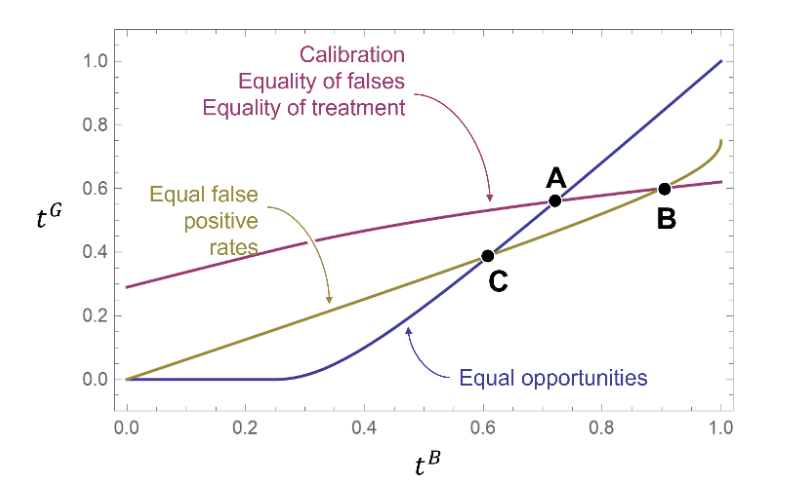
\includegraphics[width=0.45\linewidth]{./img/pasmoc2_thresholds.png}
    \end{figure}
\end{theorem}